\chapter{4. Design and Implementation}

\section{Case Study: bikebump}
To test a system that handles \hlcyan{data collection, visualization, plan proposal and prioritization}, an application for improving bike lanes was selected for a case study. Using bikes to commute has been a trend through recent years though the U.S.;  one consensus shows that there was a 3\% increase in people choosing bikes for everyday transportation from 2010 to 2013 and is close to double compared to the year 2000.\cite{debra2016onemillion} \hlcyan{City investment in bicycling infrastructure is in sync with this increase in bicycling as a method for commuting, especially in dense urban areas.} \hlcyan{New York has had 400 miles of cycle path renewals} starting from the 2000s.\cite{sadik2017streetfight} The field of public health supports this by research showing investment in \hlcyan{bike lanes is efficient} compared to other public health interventions\cite{gu2016cost}.
\footnote{The study compares different health investment by the QALY value(how much money is needed to gain one persons one year of public health.) The results shows that vaccines are exceptionally cheap (\$100), bike lane investment(\$1300) is also in the cheaper side where \$6,700 is spent for Medicaid.}


\subsection{bike lanes in urban planning}
Urban planning interventions tend to be exceptionally expensive\footnote{the United States have invested \$ 350 billion in the year of 2010 \cite{musick2010public}, and 416 billion in 2016\\ \url{https://www.cbo.gov/sites/default/files/114th-congress-2015-2016/reports/49910-Infrastructure.pdf}}, yet the process for deciding which to execute is also long and tedious. Because of this slow process and cost impact, it is difficult to make the proposal creation as a learning process. In the United States, the construction cost for a highway is 8 million to 10 million USD per mile, where one of the most expensive bike lanes will cost 445,000 USD per mile.\hlcyan{Bike lanes are relatively inexpensive; the simplest ones require only paint on the road surface.} Moreover, these interventions are reversible, \hlcyan{which enables iteration through trial and error.}
\hlcyan{While some interventions, like painting bike lanes, are cheap and reversible, and thus possible to implement quickly, other interventions are more expensive and require a great deal of domain knowledge and engineering. Implementing these solutions will inevitably a slow process.} It is difficult to design or even reach a consensus within the community. Because of the duration, ``straw polls'' may not directly reflect the demand of citizens when the construction is actually completed, especially where people tend to move frequently. Yet there are examples that the demand of such long and costly infrastructure is decreasing, since this relates to different types of transportation people use. If the trend of the number of cars decreasing continues and multi-modal transportation is accepted, light interventions such as bike lane improvements will raise the share, supported by the trend of the increase of population density, the cost impact per population will decrease.

\subsection{\hlcyan{bike way infrastructure}}

The report \underline{2012 National Survey on Bicyclist and Pedestrian Attitudes and Behaviors} shows that collision with cars is the top factor of bicyclists injury\cite{schroeder20132012}, so it is crucial to clearly separate cars and bicycles. The second(`falling') and third(`road not in good condition') cause could also be reduced by having a separate bike lanes. Research shows that protected bike lanes reduces possibility for injury in to half.\cite{teschke2012route}

Over 36\% within the population of Netherlands chose bicycles as their main mode of transportation. Relative to other countries, the Netherlands had always been keen investing bike infrastructure, even times when urban planning was aiming for a car-centric society. Investment for bike way improvements started to rise again around 1970 coupled with a protest movement to prevent children killed by car accidents. Today Amsterdam is known to be the most bike friendly city, yet there is no single solution that makes bikes this popular, this is again an example of Lessig's four elements of constraints in human behavior. For ``code'', it is easy to think it has rich bike lane infrastructure which is well connected. Moreover, the Netherlands has flat and high density geographic characters that well suits bicycle commute. ``Law'' constrains all urban planning to be fully accountable for bike lanes. Also the legislation is unfavorable for car which need to compensated most of the damage if there is an accident.  
\section{Current method for changing bike related infrastructure}
The Transportation Improvement Program is a federal requirement for each state listing improvements for all transportation needs. This is the standard throughout the U.S. and bike lane improvements are included.


\begin{figure*}[!htb]
  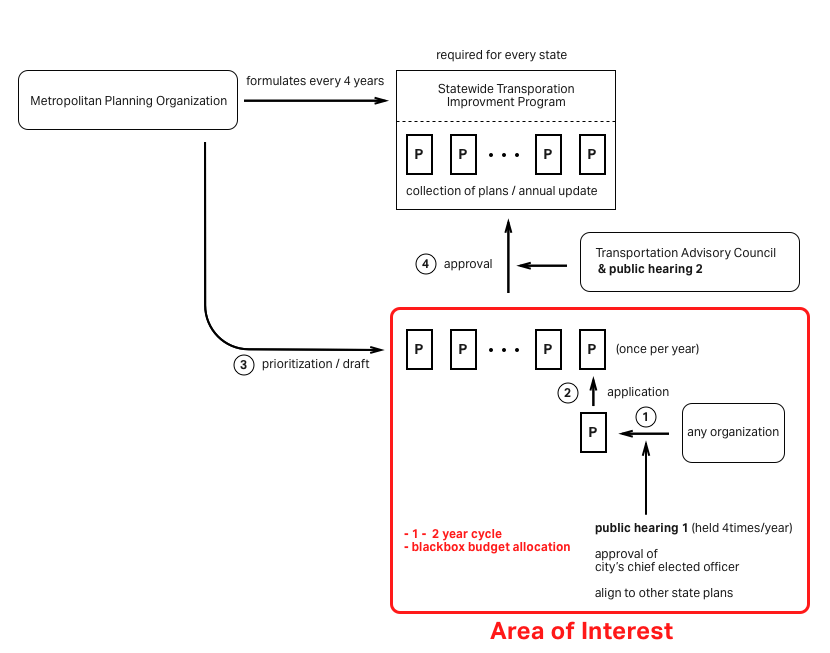
\includegraphics{chapters/4/fig/tip_process.png}               
  \caption[TIP process]{TIP(Transportation Improvement Program) required by each state. \url{https://www.gpo.gov/fdsys/pkg/USCODE-2011-title23/html/USCODE-2011-title23-chap1-sec135.htm} 
  }
  \label{fig:tip_process}
\end{figure*}

\begin{enumerate}
\item The process starts with the city level being required to have least one public hearing, and the approval of the city's mayor. This needs to be aligned with the state level manifesto.
\item After meeting the city level criteria, it is scrutinized by the local office of the Metropolitan Planning Organization(MPO). The MPO evaluates and engineers the proposal into an executable plan.  The MPO also prioritizes the plans.
\item The list of plans undergoes a second public hearing and discussed with the Transportation Advisory Council.
\item Once approved, the proposal will be listed into one plan inside the Statewide Transportation Improvement Plan.
\end{enumerate}

\begin{figure*}[!htb]
  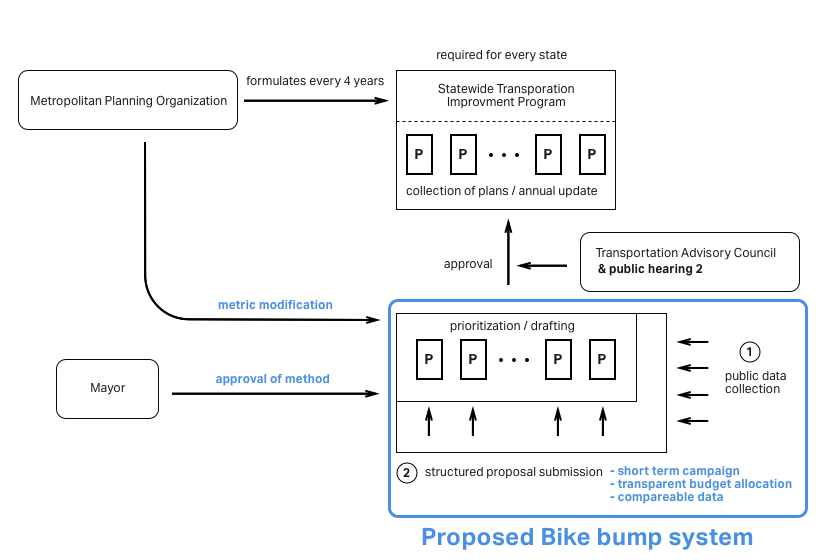
\includegraphics{chapters/4/fig/proposed_process.png}               
  \caption[proposed process]{The proposed method using bikebump trying to fit the current system. The Transportation Improvement Program (TIP) is a federal requirement for each state to compile
a list of executable improvements regarding transportation issues. The top of the pyramid from the previous includes the Metropolitan Planning
Organization and the Mayor (city CEO), given a roll of approval (which is no different from another single vote) and metric modification and engineering
of plans. The improvement plans that was generated and prioritized by bikebump will undergo one last process of being approved by the
Transportation Advisory Council which also tied to a public hearing.
} 
  \label{fig:proposed}
\end{figure*}

Other processes, such as the Cambridge Participatory Budgeting project is capable of assigning budget to road infrastructure improvements. The current method provides a way to submit an idea to any given point of the city. The ideas are based on subjective comments and no cost estimation is there, with no data to support the claim. Figure \ref{fig:proposed} shows the alternative method using bikebump. \hlcyan{Compared to present systems, the main differences are:}
\begin{enumerate}
  \item Bikebump presents a method for collecting behavioral data in the urban environment
  \item Bikebump offers a method for planning ideas from individuals
  \item Bikebump provides a method for approval for mayors
  \item Bikebump gives planning organizations ways to modify metrics and meet with longer term goals that should be consistent with previous settlements and plans
\end{enumerate}


\clearpage

\section{Implementation Overview}

This section goes through the implementation and techniques used for developing the application. The application is based on modern browsers, which recently extend the capabilities that were limited to mainly text and images. The WebRTC (Real Time Communication) is a series of protocols and APIs specifically for capturing audio and images and uses them as inputs without plugins. The bikebump application leverages this technology to capture sound data. FFT will be applied to get the frequency distribution of the called Web Audio API,

\nameref{appi:api} provides the extensive list of used APIs for developing the application.

The application is structured in the form of a web application, of which the components are: the database; back end server; front end client. The database is a NoSQL, which stores data as a giant JSON data. To reduce the number of requests and efficient data transfer, the database contains some redundancy in memory.


\subsection{Definition}

The following are definitions for certain elements that make up the application.

\textbf{DING}

A DING is a spatial representation of a ring bell report. It defines the geofence of the ding, with a center geolocation and radius. It also holds information for each report, which is the timestamp, user's ID, and the ``good''/``bad'' value based on the study protocol. If there is a road near the center location, it will also contain the road's identifier and distance from the closest point of that road.


\textbf{ROAD}

A ROAD is a geometrical feature that is returned by the Vector map API call. A newly created ding will find the closest road registered in the OpenStreetMap database and geometrical features will be copied to the bikebump database. When creating an improvement plan, users will first need to choose which


\textbf{COMMUTE}

A COMMUTE is series of GPS location data, to know the whole path of each ride session. Raw GPS data has a tendency to bounce and contain noise, so it will be processed to match the road network in OpenStreetMaps.


\textbf{BIKE COINS}

BIKE COINS are the \hlcyan{tokens} for deciding which intervention to prioritize. Each user will initially receive 100 BIKE COINS, which can be distributed by the user's choice.

\textbf{IMPROVEMENT PLAN}

An IMPROVEMENT PLAN is a combination of a CONTEXT and a SOLUTION. This method of having a separate list of where (CONTEXT) and what (SOLUTION) and combining them is taken from Christopher Alexander‘s methodology of \underline{The Pattern Language}. \cite{alexander1977pattern}


The method of defining patterns (a recipe what to do in order to come up with an outcome) and apply them to common cases is widely used in the realm of software engineering as design patterns. 
\footnote{Although Alexander himself claims that “design patterns” in software is different to what he had created, since the patterns are distinctive, having no interrelation between them. \url{https:// www.youtube.com/watch?v=98LdFA-_zfA}
}

Each IMPROVEMENT PLAN holds information of how many BIKE COINS it requires to be counted as a community approved plan. This number can be calculated using the SOLUTION‘s type and unit cost, multiplied by the length of the road.


\textbf{SOLUTION}

This is the execution instructions for a possible plan, such examples are creating Bike Boxes and painting the lane with green paint. This is separate from the CONTEXT focusing on only what to do for a road, equivalent as the patterns in the Pattern Language. Information that is included in one solution is name, description, type and unit cost. The type is used to differentiate the solution needs to account the length of the improvement or not. For example, a Bike Box will only be needed for one intersection, where painting a lane in green will differ with the total length.  The unit cost is how many BIKE COINS would be necessary per unit, which is defined by the type. The unit cost will be connected to the cost of the intervention. The cost will include but not limit to monetary cost, since some solutions will be politically difficult even in relatively cheap interventions.

For the experiment, three solutions where provided  (Table \ref{tab:solution}).

\begin{table}
  \centering
  \begin{tabular}{|c|c|r|}
  \hlcyanine
    SOLUTION & type & unit cost (m) \\ \hlcyanine
    Green Paint & road & 25\\ 
    Bike Box & intersection & 320\\ 
    Plastic Polls & road & 75 \\
    \hlcyanine
  \end{tabular}
  \caption[solutions]{Solutions provided for Experiments.
    Values are estimated by material cost. Dimensions are taken from the
    Urban Bikeway Design Guide\cite{national2014urban}. Green Paint is
    \[5ft (W) * 2 (both sides)\] 
    BikeBox is
    \[12ft (W) * 16ft (H) \]

    Cost estimation can be done here 
    \url{http://www.asphaltkingdom.com/parking-lot-paint-calculator}

    Plastic polls are put in 2m pitch with each costing \$150
    \cite{aarian2016want}, therefore
    \$75 for each meter. 
  }
  \label{tab:solution}
\end{table}

Green Paint is painting the bike lane into green. The material has varieties such as ordinary paint, Durable Liquid Pavement Markings(DLPM)\footnote{acrylic resin}, and thermoplastic. Changing the pavement to a different colored material has the same effect. The budget calculation is done using the least expensive using ordinary paint. This tends to worn out fast, which is also easy to erase it.\cite{national2014urban} A Bikebox is a marking for intersection to have a place for bikes stop before the cars. This makes it easier for bikes to turn especially to the left \footnote{in the United States, which is right side traffic.} The material is identical to the Green Paint intervention. Plastic Polls are tubular markers that separate the car lane and the bike lane. It is one of the cheapest intervention to create a protected bike way. 

\textbf{CONTEXT}

The CONTEXT is a segment of a road which a SOLUTION will be applied. The system enables the users to select which part of a road they would like to improve. The segment will include information of the length to by multiplied by the unit solution cost, if applicable.


\section{Interface}

The application has five major views: recording view; map view; vote view; improvement list view; improvement creation view.
The top navigation bar guides the user to jump between the views.


\subsection{Record view}

\begin{figure}[!htb]
  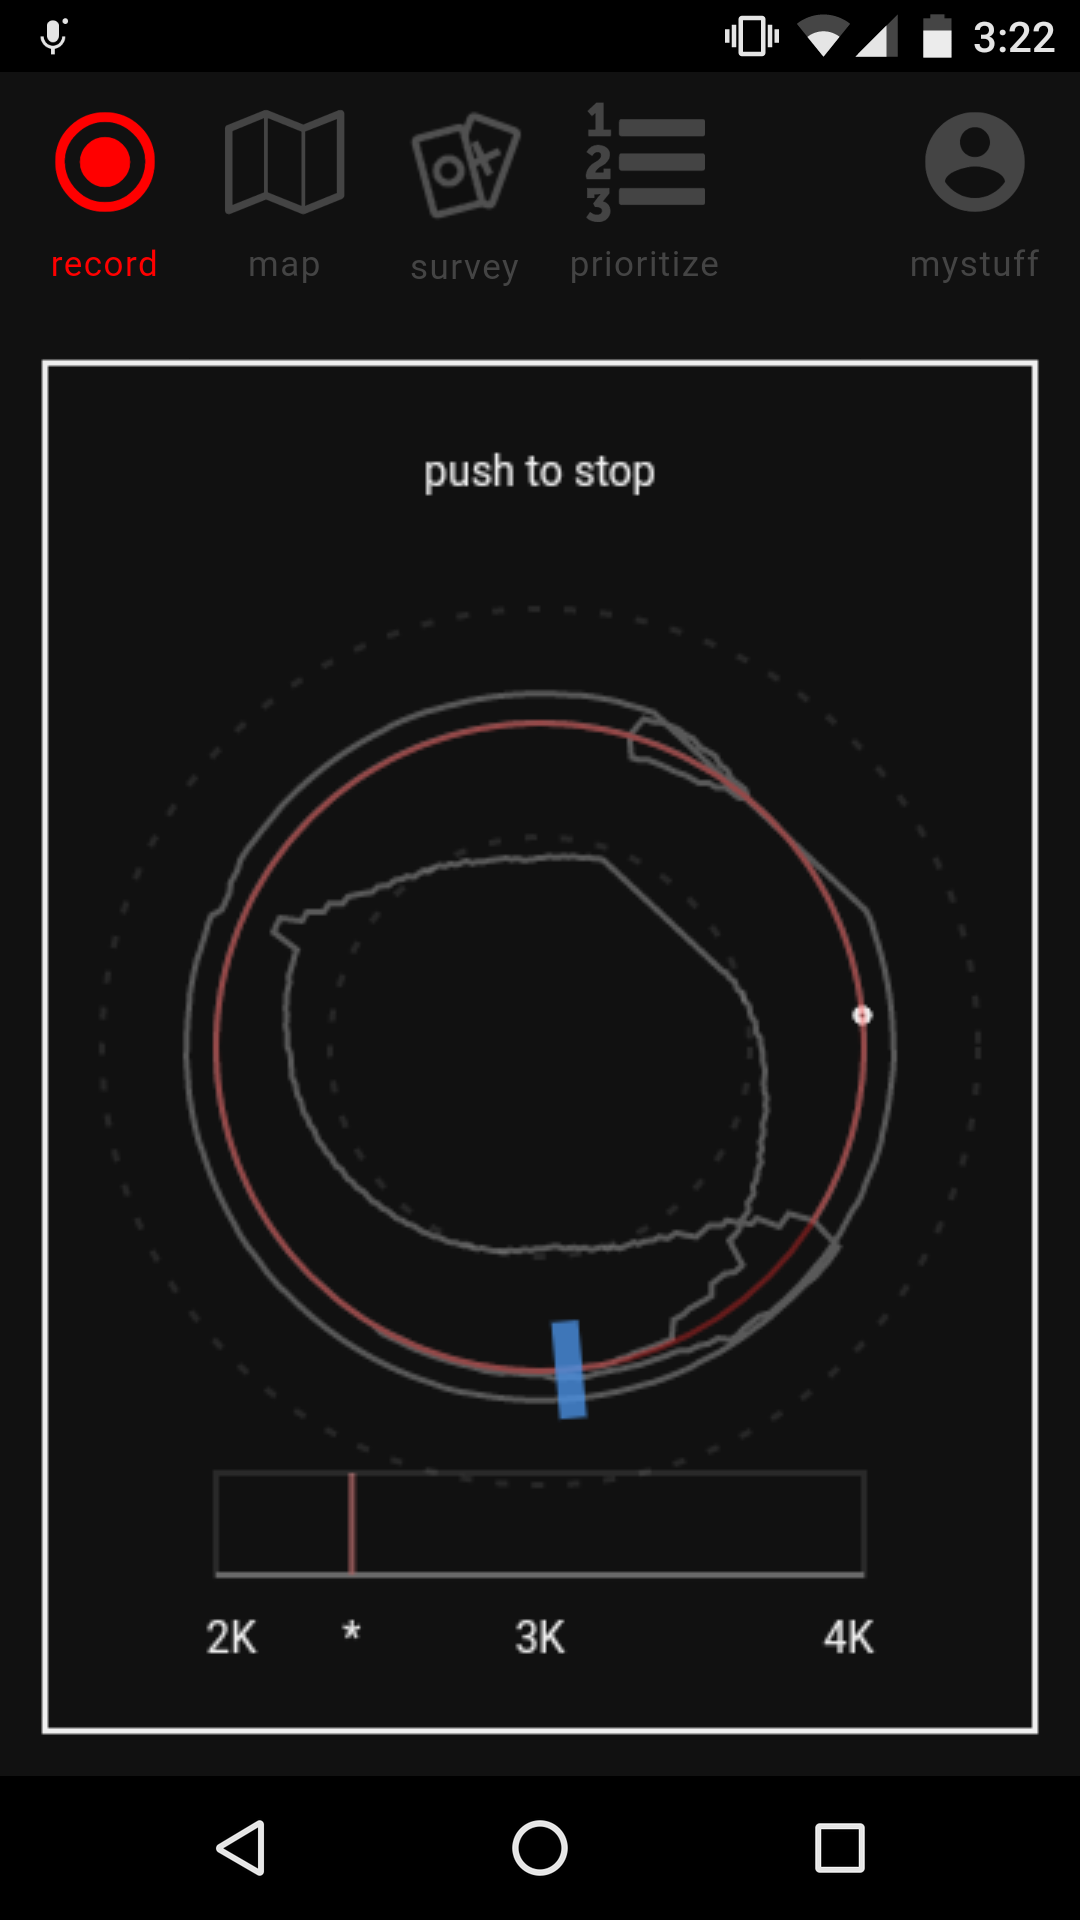
\includegraphics[width=0.6\textwidth]{chapters/4/fig/interface_recording.png}
  \caption[interface: Record]{recording view}
  \label{fig:interface_record}
\end{figure}

Figure \ref{fig:interface_record} is the main view when users ride their bikes and record events. After signing up to the system, the user will go though a process to registering their bell's target frequency's peak amplitude and duration of a ring as a threshold of detection. Users are able to re-configure the bell values by user settings. The primary function is to \hlcyan{detect the ring, register the time and location and report those to the server}. Based on  given  data  from  the  calibration, the application looks into the target frequency and validates two thresholds: the slope through the adjacent frequency values; the duration that slope threshold persisted (time limit). Refer to\ref{appendix:time} for details on the method of ring bell detection. The initial detection will store two things in memory: the latest geolocation and a sound of 4 seconds before the detection.
\footnote{The recorder holds a data array with constant length and stores each sound input, overwriting the data each time
it is full. This data array will be developed when saving as an audio clip. To exclude the first part of the detection, the system will record from
-5 seconds to -1 seconds relative to the detection.}

\hlcyan{If detection occurred once and no detection for the next 4 seconds, the application flags the report to be ``bad'', if there is more than one detection within the 4 second window the report will be labeled ``good''.}After the four seconds, the application will submit the geolocation of the first location, sound data and ``good''/``bad'' label to the server, and return to the initial state. The users will be notified about this one ring is ``bad'' and more than twice means ``good'' protocol beforehand.

The interface uses an animation frame to show the detection and the label data “good” or “bad,” with a circle orbiting the 4-second detection interval. For safety reasons, when recording, other buttons are disabled to prevent user input. Also, while recording, the application will periodically query the geolocation and store “bread crumbs” of location.

\subsection{Map View}

\begin{figure}[htb]
  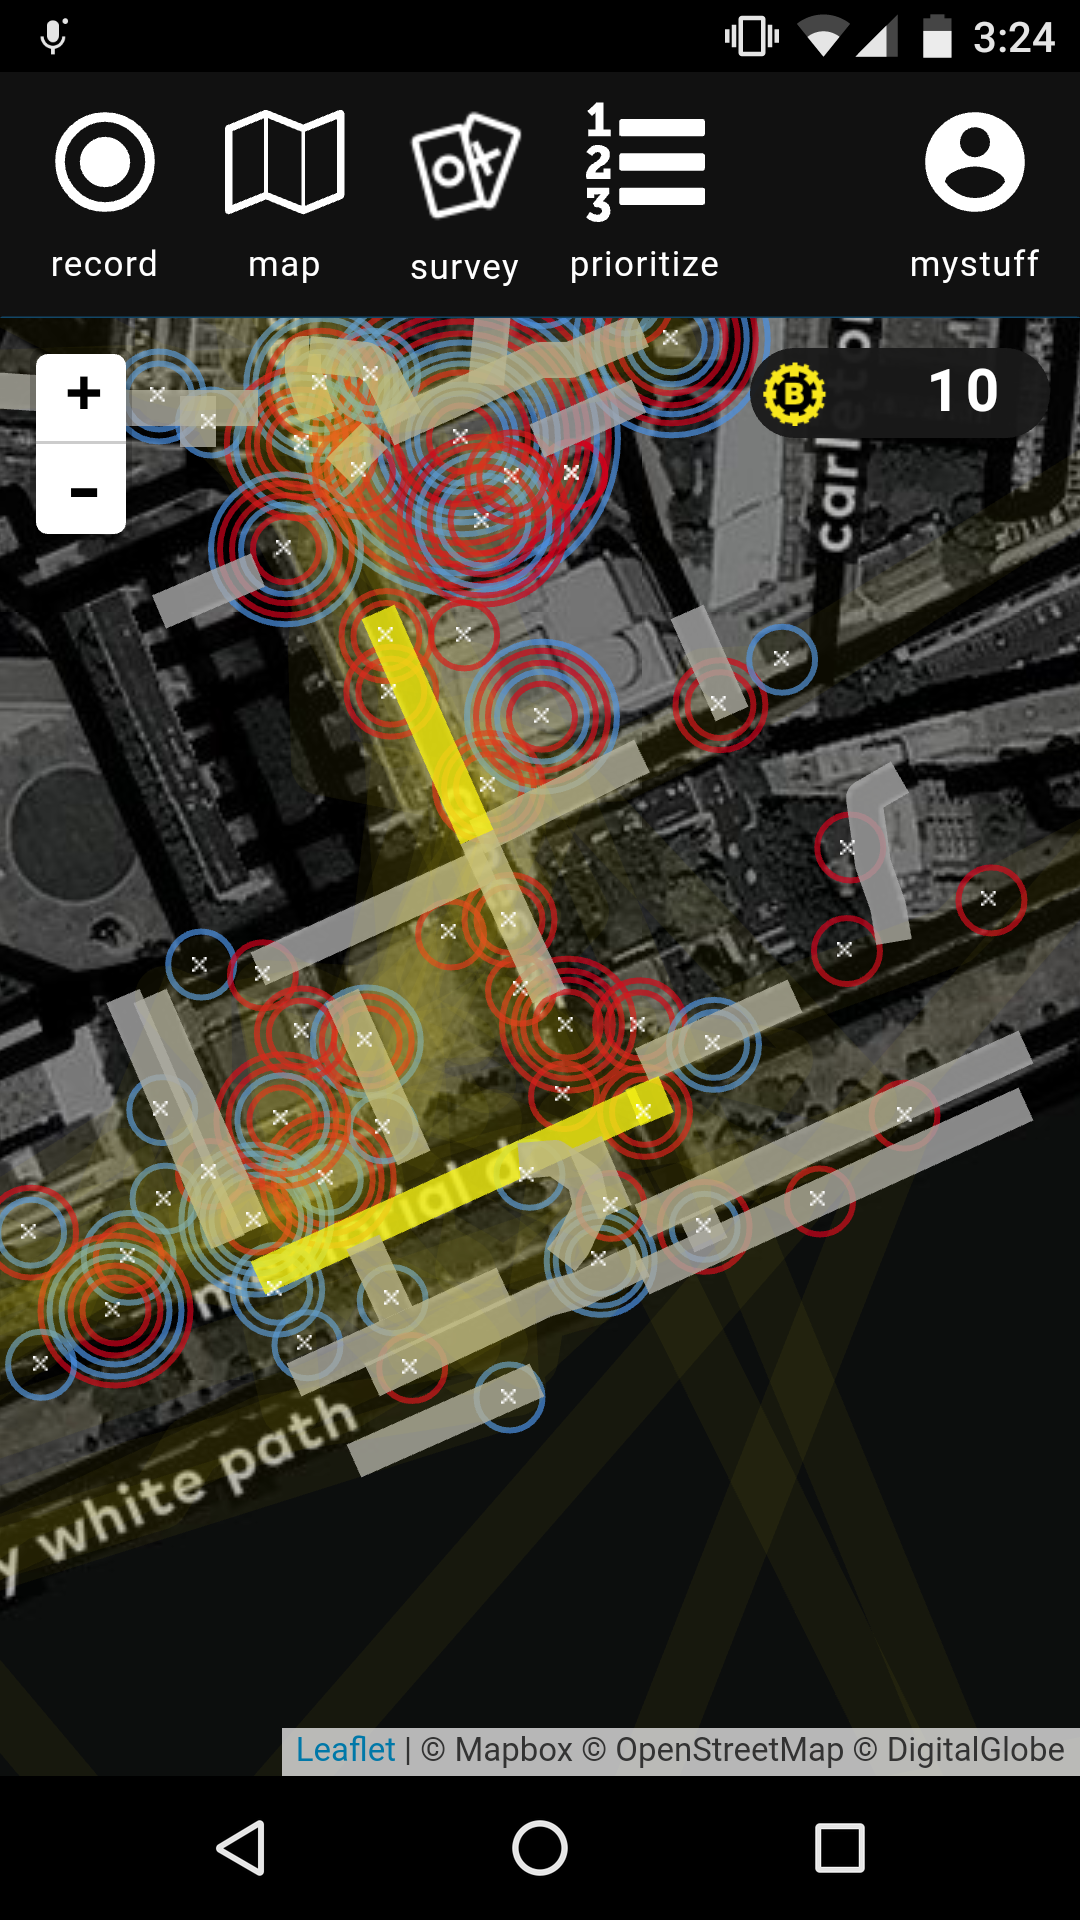
\includegraphics[width=0.6\textwidth]{chapters/4/fig/interface_map.png}               
  \caption[interface: Map]{Map view}
  \label{fig:interface_map}
\end{figure}

\begin{marginfigure}[{0cm}]
  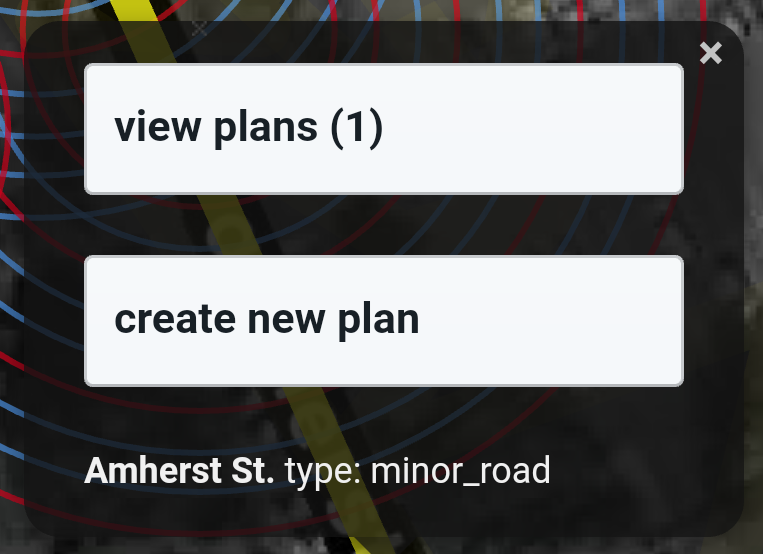
\includegraphics{chapters/4/fig/interface_popup.png}               
  \caption[interface: Popup]{a pop-up navigator linked to creating or
  voting to IMPROVEMENT PLANS}
  \label{fig:interface_popup}
\end{marginfigure}

The map view (Figure \ref{fig:interface_map}) visualizes the data obtained by users. The visualization includes geolocation data of people's DINGs, highlighted roads that had one or more closest dings, and the commute paths people took. Yellow road segments indicate that there was at least one improvement plan submitted by any user. The roads have pop-ups (Figure \ref{fig:interface_popup}) that link to options to existing improvement plans or the improvement creation view.

\subsection{Survey View}

\begin{figure}[htb]
  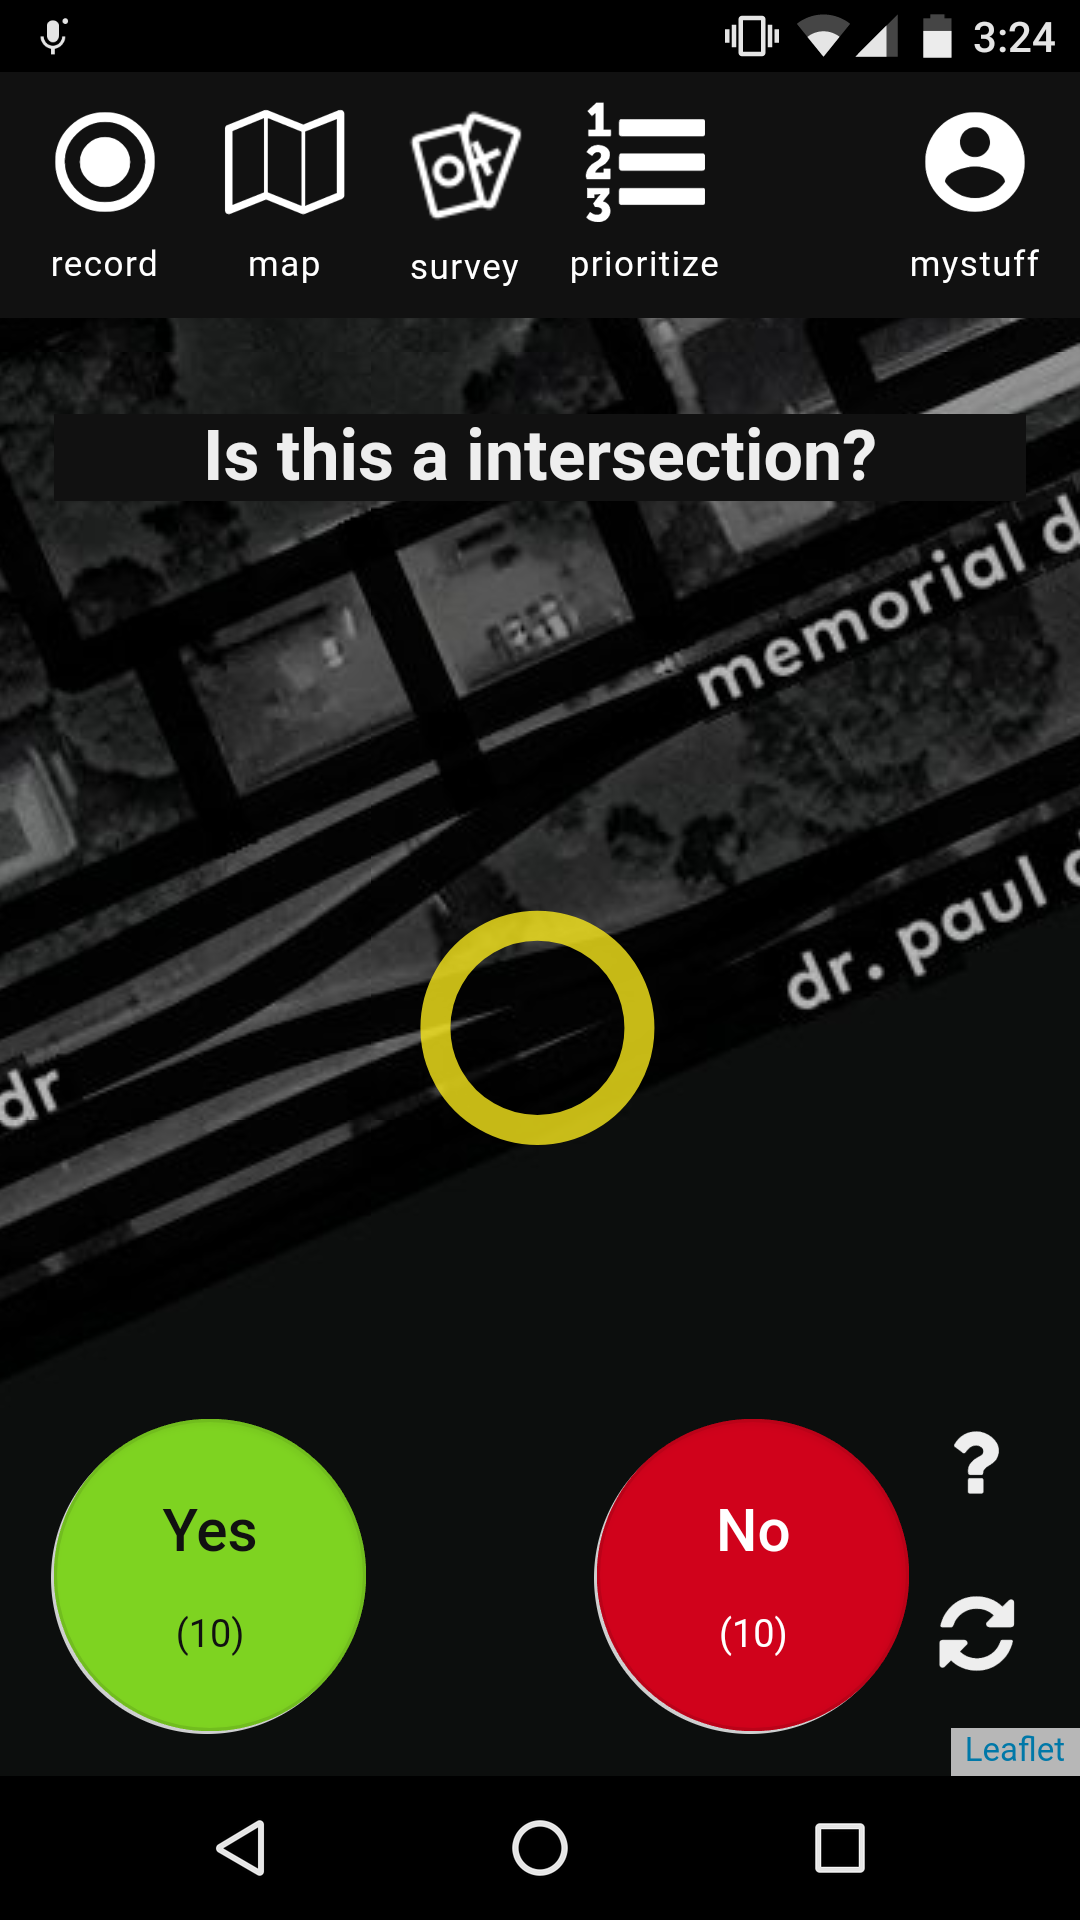
\includegraphics[width=0.6\textwidth]{chapters/4/fig/interface_survey.png}               
  \caption[interface: Survey]{Survey view}
  \label{fig:interface_survey}
\end{figure}

The survey view asks the users follow up questions to complement their ding reporting. There are two purposes for having this feature, thus two kinds of questions. The first purpose is to collect information that does not exist in the map data such as OpenStreetMap (OSM). OSM data does not include information about specific conditions
about the bike lane, for example, painted in green, or separated with plastic bollards.
\footnote{
 some Path network includes information on the existence of a bike
 lane or an attribute indicating it is a cycle path yet the data have no
 guarantee that it is updated timely.
} 
The type of questions that serve this purpose is for retrieving information on the current condition. For the experiment, these questions were:

\begin{enumerate}
  \item Is this place an intersection?
  \item Was there a separated bike lane?
\end{enumerate}

Secondly, the reason for the ``good'' / ``bad'' judgments varies, so it requires more information to
ask for specific reasons why the report occurred. One ``bad'' DING may be because of a pothole or a
car blocking the bike lane (occasional conditions) or no bike lane (planning conditions).

\begin{enumerate}
  \item The road was bumpy.
  \item It had a lot of tree shades.
\end{enumerate}

\subsection{Create Improvement View}

The create improvement view enables users to submit improvements to the system to be voted on by other users.
The pop-up menu that each road shows (Figure \ref{fig:interface_popup}) provides links to this view (Figure \ref{fig:interface_improvment}). 
To create an IMPROVEMENT PLAN, it is required to select one SOLUTION,
and if applicable, which range to apply for the selected road.

The user who proposes any plan will need to decide the trade off between different solutions and ranges, \hlcyan{because choosing expensive improvements will be difficult to approved as a community.}


\begin{figure}[!htb]
  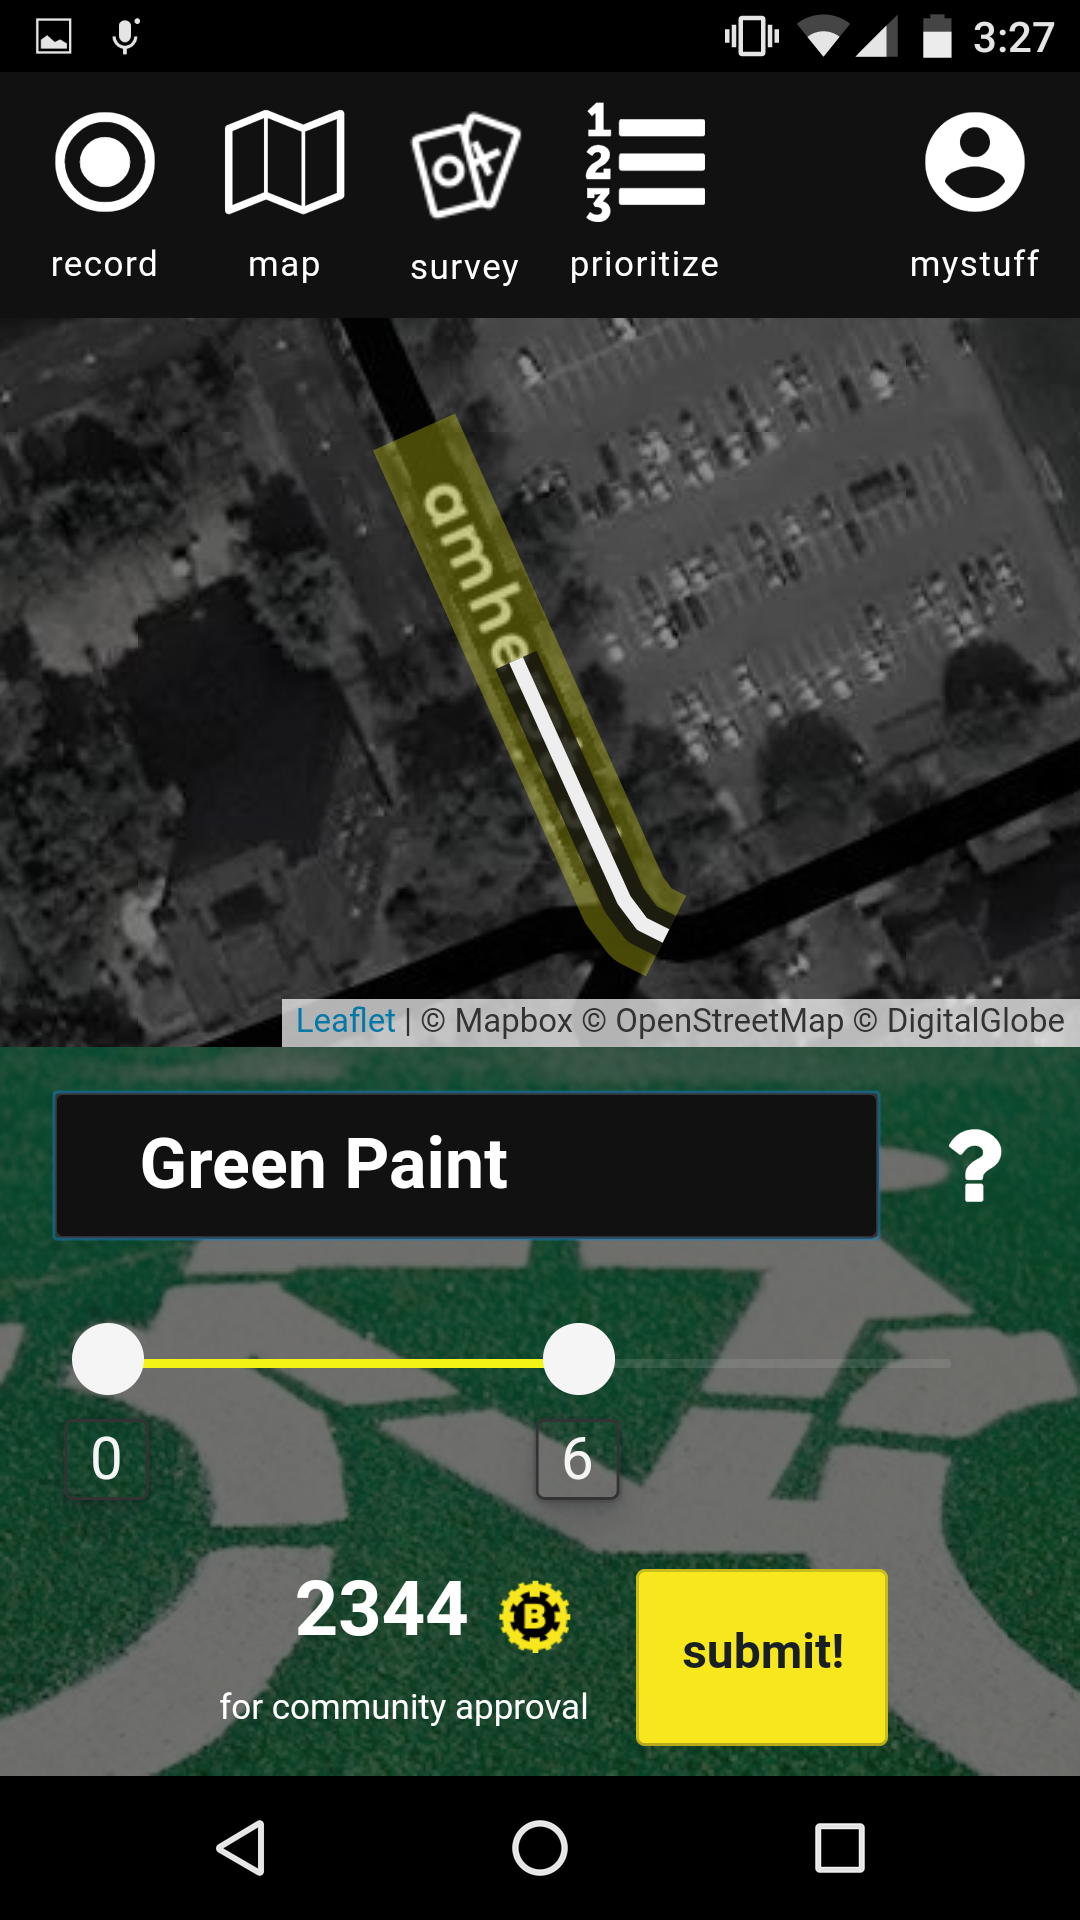
\includegraphics[width=0.6\textwidth]{chapters/4/fig/interface_solution2.png}               
  \caption[interface: Survey]{Survey view}
  \label{fig:interface_improvment}
\end{figure}

\subsection{Vote View}

Each IMPROVEMENT PLAN will have a vote view. It provides the interface to distribute points for the segment. It is a four-choice question, with the option to give 0, 10, 20, and 50 BIKE COINS to the target plan. The application permits the user to vote for their own IMPROVEMENT

\begin{marginfigure}
  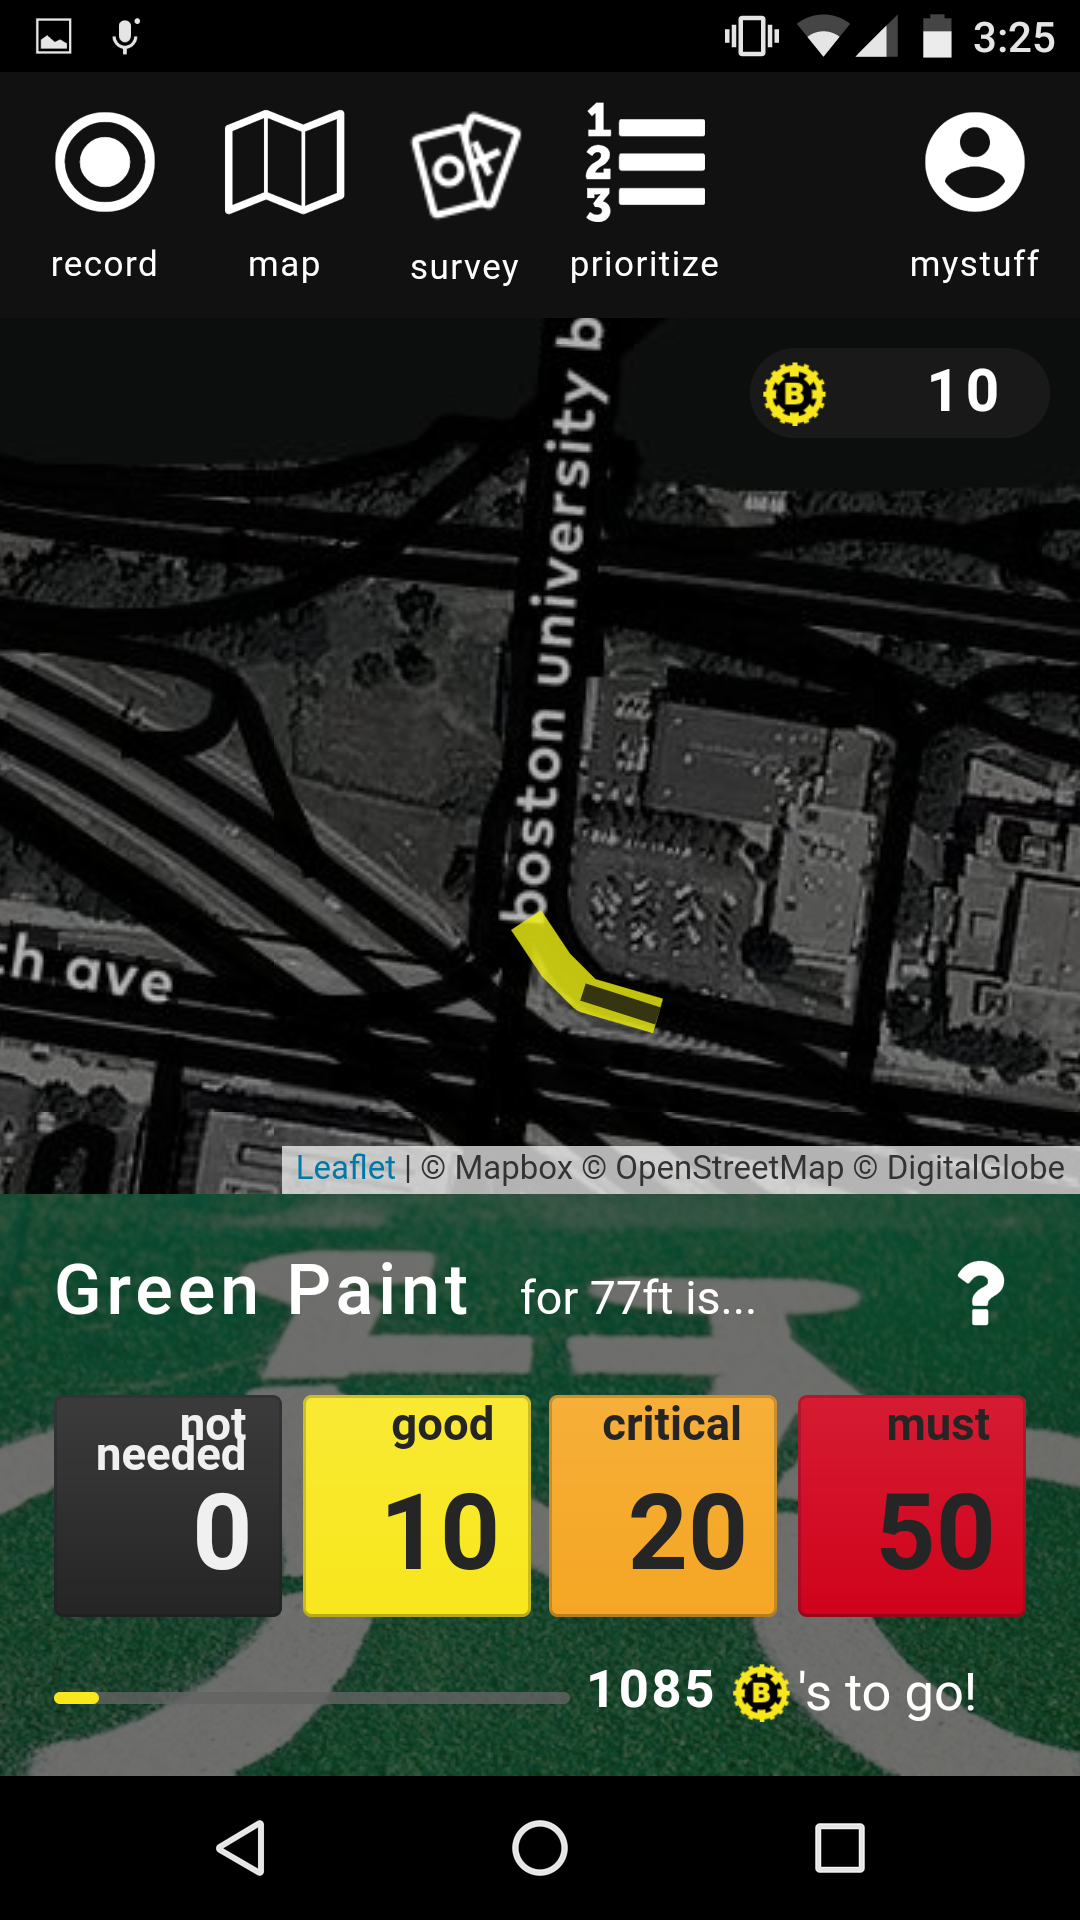
\includegraphics[width=0.6\textwidth]{chapters/4/fig/interface_vote.png}               
  \caption[interface: Vote]{Vote view}
  \label{fig:interface_vote}
\end{marginfigure}

\subsection{Improvement List View}

\begin{figure}[!htb]
  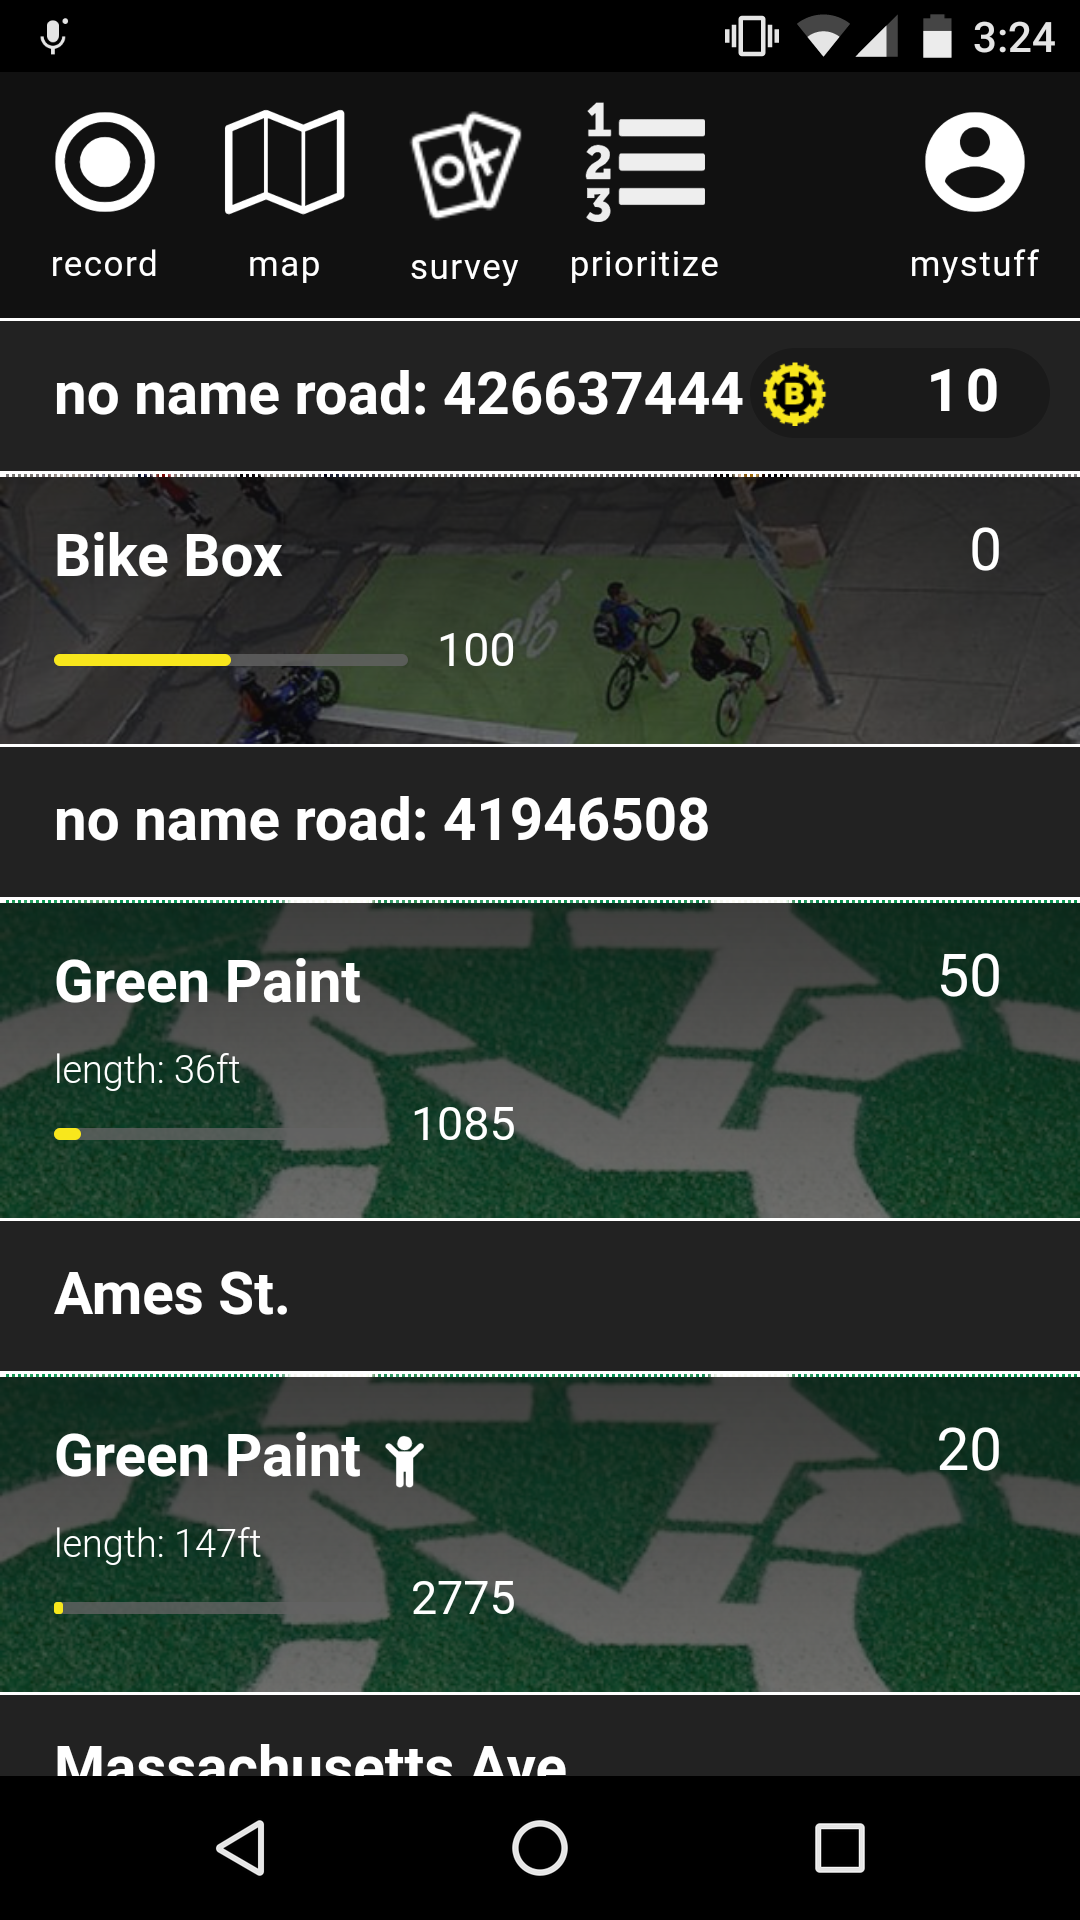
\includegraphics[width=0.6\textwidth]{chapters/4/fig/interface_list.png}               
  \caption[interface: Improvement list]{Improvement list}
  \label{fig:interface_list}
\end{figure}

The improvement list is the where users can see a sorted list of improvements. Individual improvements are categorized by associated roads and the list is first sorted by the sum of BIKE COINS gathered to the road. Inside a single road category, it is sorted by the number of achieved BIKE COINS for the single IMPROVEMENT PLAN.


\section{Experiment Setting}
A human subject test was conducted to examine the functionality and effectiveness of the prototype. Refer to \nameref{apph:human} for the complete consent form.

A total of 20 people had been recruited by email and social media posts; the users’ demographic was students and individuals from local
 bike advocacy bike advocacy groups. Out of the 20 participants, five were female subjects. Each test had one participant.

Three participated using a bike sharing service 
\footnote{Hubway \url{https://www.thehubway.com/}}
others used their bike.
12 people used the bell provided, and none owned a smart phone mount. \hlcyan{Every user was required to calibrate their bells before starting the experiment.}
The experiment was conducted during the day, without rain, time slots were 9:30, 12:00, 14:00, and 15:00.

Each test took around 1.5 hours. The experiment had four steps.
The first was the orientation, where the examiner introduced the objective of the user test, gained subject's consent,
asked for the initial survey, showed how the application works, and talked about the route of the on-bike experiment.


\begin{figure}[htb]
  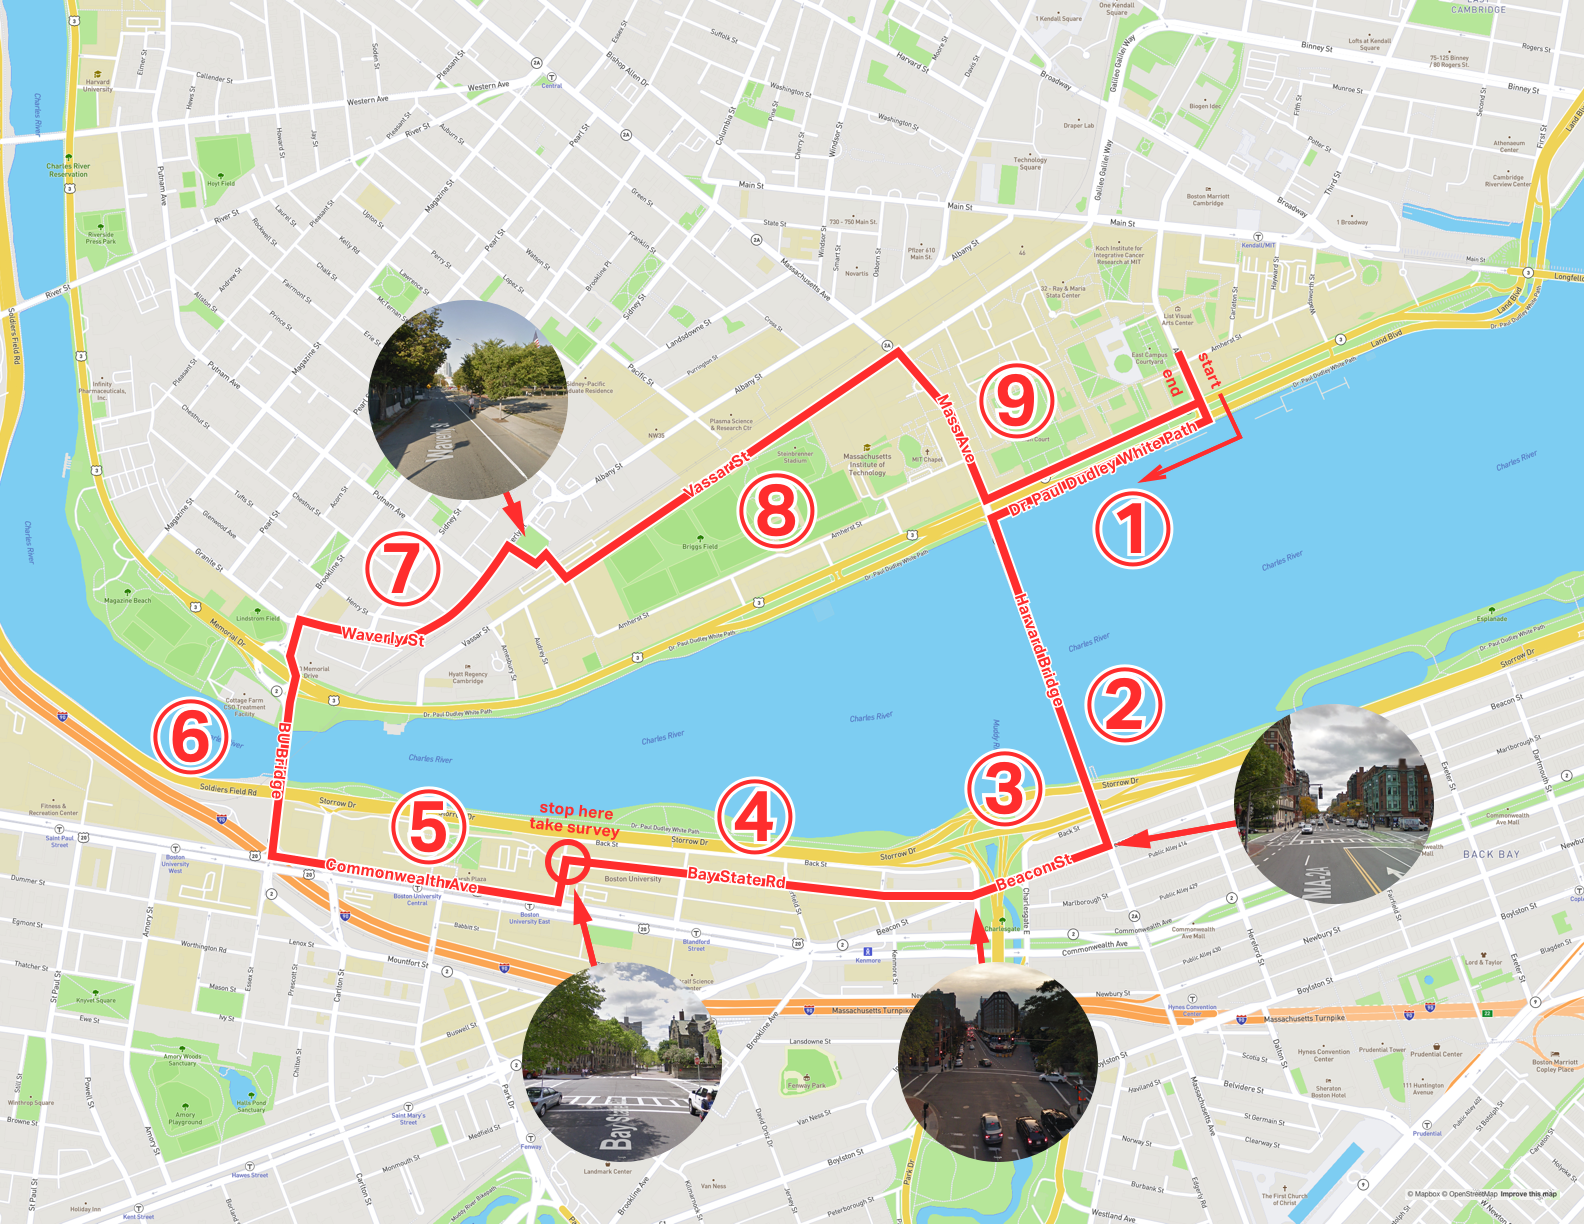
\includegraphics[\textwidth]{chapters/4/fig/fixed_route.png}             
  \caption[fixed route map]{route for the experiment}
  \label{fig:route}
\end{figure}

The second step was to have the users ride the bike, with the application running. Figure \ref{fig:route} is the path that was asked for subjects to take. The start location was the entrance of MIT Media Lab heading towards the Charles river turning right taking the Dr. Paul Dudley White Path \hlcyan{(Map 1)}. This path was renewed in 2017, with a bi-directional cycle path, which is rare in Cambridge. The route makes a left turn to take the Harvard Bridge(Map 2), which does not have a dedicated bike lane. Car traffic is relatively high since there is no light until the end of the bridge. The intersection of Harvard Bridge and Beacon Street(Map 3) is infamous for having accidents and is considered one of the most dangerous crossings.
\footnote{a cyclist died hit by a tractor trailer in 2015
\url{https://www.bostonglobe.com/metro/2015/08/07/woman-bicyclist-injured-apparent-collision-with-vehicle-back-bay/zsjWYLZIZ324kSkmbjOaWM/story.html}}
In response to the number of accidents, the city of Boston
modified the lane structure for the crossing and Beacon Street. Proceeding to Beacon Street, the route takes a slight right for Bay State Road(Map 4). Park Driveway crosses Beacon Street close to this intersection, which is also close to the intersection of a major cross down Parkway, Storrow Drive. Bay State Road is a one-way road with less traffic but no bike lanes and an arch of tall trees on both sides. The users were asked to take a survey using the application at the intersection of Back Street. Taking a short left turn is Commonwealth Avenue(Map 5), which is a wide multi lane road that is a part of an arterial route. Despite the wide road and fast traffic, there is no separated bike lane. Subjects then took the BU Bridge(Map 6) heading back to Cambridge. Over the weeks of experiments, this BU Bridge was closed to cars, allowing only pedestrians and bikers to cross.
\footnote{
Boston Globe reported the happy comments from the cyclists, right after the shutdown. 
\url{https://www. bostonglobe.com/metro/2017/07/28/for-cyclists-bridge-closure-like-heaven/bBWnlm00ROV7LfZW0w7f2O/story.html}
}
The BU Bridge ends with a roundabout that does not have lights or separated bike lanes. The route turns left after the roundabout to Waverly Street(Map 7), a thin single lane street. The path turns right before the park to take Vassar Street(Map 8). Vassar Street has a dedicated bikeway at the same level of the sidewalk. The route returns to Massachusetts Avenue(Map 9) crossing MIT's main entrance. This part is often crowded with tourist buses and many pedestrians crossing. It is also close to the bridge, which the drivers rush to catch the light with high speed. Lastly, the route heads back to the origin using the same path, but the opposite side. There is a lengthy discussion on bikes riding on sidewalks, and the law is different depending on the area. Massachusetts law permits bikers to use the sidewalks if the local city permits them to do so.
\footnote{Massachusetts General Laws PartI Title XIV Chapter 85 Section 11 B
\url{https:// malegislature.gov/Laws/GeneralLaws/PartI/TitleXIV/Chapter85/Section11B}
}
The city of Cambridge does not ban bicycles from using the sidewalks on Memorial Drive.
\footnote{Sidewalk Bicycling Banned Areas.
\url{http://www.cambridgema.gov/CDD/Transportation/gettingaroundcambridge/bybike/rulesoftheroad.aspx}
}

This on-bike test was designed to take approximately 30 minutes. Within the experiment, users were required to stop and take an in-experiment survey.

\textbf{After the users had come back from the trial, There is a 10min discussion regarding the data collection phase, mainly talking general feedback about the app and vocal review about the fixed route.
The experiment will then jump to demonstrate how to submit a proposal plan. Users will select a ROAD segment that he or she felt it is worth to have a intervention in the map view. Then bikebump will guide the user how to add a IMPROVEMENT PLAN by selecting the solution type and if applicable the domain within that ROAD segment. The subject will observe the submitted plan and give out BIKE COINS as much as the user thinks the proposal is necessary. The user will look up other proposal created by other users and vote for most favorable plans. Lastly, it will have another discussion focusing on improvement submission and how it is different from the first data collection phase.
}

\clearpage

\section{Results}

\begin{figure*}[!htb]
  \includegraphics{chapters/4/fig/result_map.png}               
  \caption[result map]{result of data collection} 
  \label{fig:map_result}
\end{figure*}


\subsection{Quantitative}
\textbf{Accident report comparison} \\
Within the fixed route, \hlcyan{there were 186 DINGS, and 283 bad reports within the 20 trips of the same route
  \footnote{The DING number is DINGs that had more than one bad reports, so the DINGs only with good DINGs are excluded. Each ``bad'' DING had an average of 1.52 ``bad'' reports.}

Data from Boston and Cambridge Police\footnote{
achieved by Cambridge open data portal \url{https://data.cambridgema.gov/Public-Safety/Police-Department-Crash-Data-Historical/ybny-g9cv}
} shows there were 30 accidents reported from 2002 to 2016. The DING reports captured 73.3\% (22 location) of these locations within a 15m radius, and the total likelihood of a user reporting a ``bad'' report that had a accident is 13.78\% \footnote{Given that there were 283 ``bad'' reports and a total of 39 ``bad'' reports that include an accident.} If set the DING radius to 20m\footnote{The GPS accuracy is claimed to be 4.9m. The application requests the GPS value every 5 seconds, when the average bike speed is 4-5m/second. By these numbers the maximum error radius is between 14.9m - 17.4m}
, 96.6\%\footnote{DINGs that included an accident had an average of 1.77 ``bad'' reports, which is larger then the total average.} of the accidents were covered. 

}

\textbf{Ambient sound noise and `bad' report correlation} \\
for the details on the how to process the see \nameref{app:urban_sound}.

The model prediction accuracy to predict ``good'' / ``bad'' was 60\%. Using the selected method\cite{piczak2015environmental}, the sound clip data did not show significant relation with people's reports.

% \tectbf{BU Bridge before and after}\\
% The tendency of the report changed radically after the bridge shut down.

\subsection{Qualitative}
A summary of the replies for the after-bike discussion follows. The next section will discuss the subject's response in detail:
\begin{itemize}
\item None of the people knew the standard process to change a road.
\item Most of the people recognized that this could be useful to learn the collective opinion and may be able to replace the current system without modification.
\item People said, ``bad'' reports were often a moment or a point, where ``good'' reports were often a continuous feeling. \hlcyan{The behaviour reporting ''good`` locations varied by users. Some only reported once though the good region\footnote{Often the when they first recognized the feel ``good''.}, while some reported periodically.}
\item The majority of subjects felt awkward when ringing the bell when there was someone in front.\hlcyan{One user said they hold back reporting when they saw a police officer running ahead of him.}
\item Participants understood there were two distinct processes, and felt it was useful to have them integrated into one. \nameref{appc:afterquestions} question 8. \hlcyan{When introduced to the feature that let's users submit users, the majority of the users first looked at the places that they felt most danger and looked at the DING reports. This is a indication that the visualization view worked as a verification. One subject reported the distinction comes from the logical procedure of the two phases. The reasoning of a improvement plan comes from the observation of the report.}
\item The interview had a section that discussed the two usages of the application. One is open access where the citizen can download and use whenever they wish, create improvement plans, and vote for them without any limitation. The second possibility is the city concentrating to a specific road they think they needs to be improved and setting predefined improvement plans, and then being told by the city to concentrate on a particular route. \hlcyan{Two users preferred the fixed route supervised by the city, where the others preferred complete freedom.}
\end{itemize}

\section{Evaluation}

\begin{figure*}[!htb]
  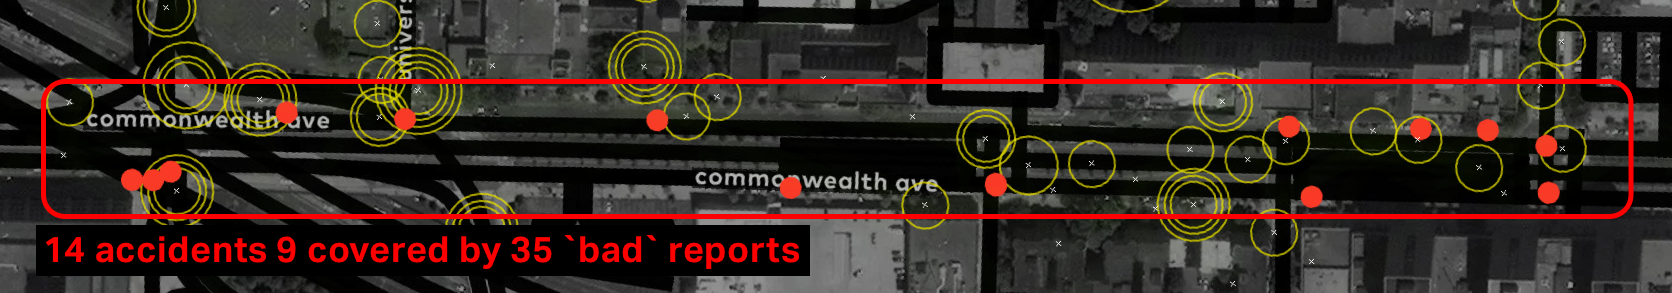
\includegraphics{chapters/4/fig/overlap_commonwealth.png}               
  \caption[dangerous road]{Figure \ref{fig:map_overlap_commonwealth} and Figure \ref{fig:map_overlap_crossing} are closeup views overlaid with bike accidents that occurred during 2002 - 2016. Yellow rings indicate `bad' dings, and red dots indicate the location that had accidents. Commonwealth avenue, had the most accidents though the fixed route.}
  \label{fig:map_overlap_commonwealth}
\end{figure*}

\begin{figure}[!htb]
  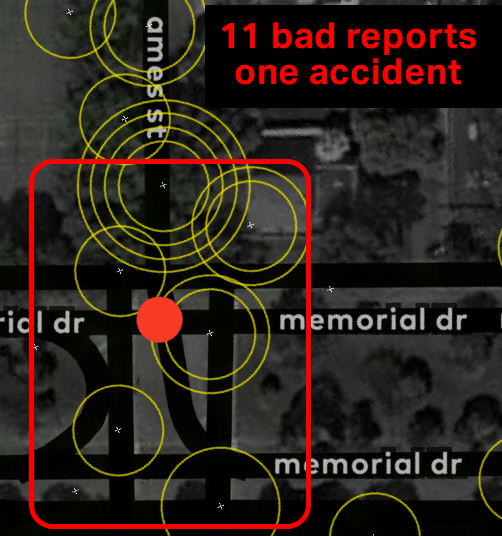
\includegraphics{chapters/4/fig/overlap_ames_crossing.png}               
  \caption[dangerous crossing at ames Street]{The crossing between Ames and Crossing was infamous between the users, with fast traffic and no eye contact.}
  \label{fig:map_overlap_crossing}
\end{figure}

\subsection{Analytical side}
\begin{itemize}
  \item Most of the people said the application functioned as intended. While there were some complaints, it was \hlcyan{unstable and hard to register a ding} when large vehicles (trucks and buses) passed. \hlcyan{People did not recognize any false positive detection\footnote{This does not mean the application was accurate, because it is assumed that users concentrate on the road, not looking at the interface while riding.}}
  \item \hlcyan{DING reports shows some alignment with accidents, while it is dependant on which route the users took. If the application was used for open access\footnote{Without concentrating on a particular path} it may be hard to gather sufficient amount of commutes from diverse bikers using the same route.}
  It is difficult and too early to say that sound clip data is a good  predictor  of  bike  accidents.  Microphones in smart phones may be optimized to filter noise, thus the very information we are interested in may be removed from the data. Future research is required for both how to gather data, as well as the method to process it.
  \item Relativeness - There were multiple times people stated they felt in danger when the bike lane disappeared. \hlcyan{The sensation of unsafeness may be a relative phenomenon, a reaction to the previous feeling of safety.} This comment is an indication that already it is a `wicked problem'
\end{itemize}

\subsection{Synthetic side}
\item Except one subject that was working in the planning sector, none knew how to propose the standardized method to submit an improvement plan to the city. \hlcyan{For students from other countries, all of them replied that they did not know even if it was their own country. This indicates that the demand for proposing a bike lane was lower than to spend effort on research.} 
\item Most people said there is no disadvantage to having a proposal layer on top of the data layer. Some stated it is better to have the analytical side and synthetic side integrated since it is easy to go back and forth, \hlcyan{while some users felt the integration of layers could be more intuitive.}
\item There are two ways to use this application in practice. A controlled engagement where the city provides the particular segment and for the call for data collection and improvement plans. In contrast, a free platform that the citizens/participants are free to collect data and submit improvement plans to their demand. Most of the participants preferred the free version, yet led to a dilemma that if it was free to use, there are very few chances to encounter that application or install it, and it may be used and dominated by serious bikers, which is exclusive and opposite from having a grassroots method.

